\documentclass[dvipsnames]{beamer}
\mode<presentation>
\usepackage{graphicx}
\usepackage{wasysym}
\usepackage{hyperref}
\definecolor{links}{HTML}{2A1B81}
\hypersetup{colorlinks,linkcolor=,urlcolor=links}
\usepackage{fancyhdr}
\usepackage{multicol}
\usepackage{multirow}
\usepackage{float}
\usepackage{amssymb}
\usepackage{scalerel,stackengine,amsmath}

\usepackage[normalem]{ulem}
\def\Put(#1,#2)#3{\leavevmode\makebox(0,0){\put(#1,#2){#3}}}

\usepackage{tikz}
\usetikzlibrary{arrows,shapes,chains}
\usetikzlibrary{positioning,decorations.pathreplacing}
\usetikzlibrary{fit,shapes.misc}
\usetikzlibrary{decorations.pathreplacing,calc}
\newcommand{\tikzmark}[1]{\tikz[overlay,remember picture] \node (#1) {};}
\tikzset{
	startstop/.style={
		rectangle, 
		rounded corners,
		minimum width=3cm, 
		minimum height=1cm,
		align=center, 
		draw=black, 
		fill=red!30
	},
	process/.style={
		rectangle, 
		minimum width=3cm, 
		minimum height=1cm, 
		align=center, 
		draw=black, 
		fill=blue!30
	},
	decision/.style={
		rectangle, 
		minimum width=3cm, 
		minimum height=1cm, align=center, 
		draw=black, 
		fill=green!30
	},
	arrow/.style={thick,->,>=stealth},
	dec/.style={
		ellipse, 
		align=center, 
		draw=black, 
		fill=green!30
	},
}
\tikzset{cross/.style={cross out, draw, 
		minimum size=2*(#1-\pgflinewidth), 
		inner sep=0pt, outer sep=0pt,color=red},
	decoration={brace},
	tuborg/.style={decorate}}

\tikzset{
	invisible/.style={opacity=0},
	visible on/.style={alt=#1{}{invisible}},
	alt/.code args={<#1>#2#3}{%
		\alt<#1>{\pgfkeysalso{#2}}{\pgfkeysalso{#3}} % \pgfkeysalso doesn't change the path
	},
}  


\usepackage{geometry}
\usepackage{appendixnumberbeamer}

\usepackage{listliketab} %make itemize env behaving like tables !
\usepackage{listings}
\usepackage{setspace}
\usepackage{color}
% General Colors
\definecolor{deepblue}{rgb}{0,0,0.5}
\definecolor{deepred}{rgb}{0.6,0,0}
\definecolor{deepgreen}{rgb}{0,0.5,0}

% Colors for Python
\definecolor{Code}{rgb}{0,0,0}
\definecolor{Decorators}{rgb}{0.5,0.5,0.5}
\definecolor{Numbers}{rgb}{0.5,0,0}
\definecolor{MatchingBrackets}{rgb}{0.25,0.5,0.5}
\definecolor{Keywords}{rgb}{0,0,0.5}
\definecolor{Strings}{rgb}{0,0.63,0}
\definecolor{Comments}{rgb}{0.4,0.4,0.4}
\definecolor{Backquotes}{rgb}{0,0,0}
\definecolor{Classname}{rgb}{0,0,0}
\definecolor{FunctionName}{rgb}{0,0,0}
\definecolor{Operators}{rgb}{0,0,0}
\definecolor{Background}{rgb}{0.93,0.93,0.93}

\definecolor{RWTHbluedark}{RGB}{0,84,159}
\definecolor{RWTHbluelight}{RGB}{142,186,229}
\definecolor{RWTHmagenta}{RGB}{227,0,102}
\definecolor{RWTHmagentalight}{RGB}{249,210,218}
\definecolor{RWTHyellow}{RGB}{255,237,0}
\definecolor{RWTHorange}{RGB}{246,168,0}
\definecolor{RWTHred}{RGB}{204,7,30}
\definecolor{RWTHgreen}{RGB}{87,171,39}
\definecolor{RWTHlila}{RGB}{122,111,172}
\definecolor{RWTHbordeaux}{RGB}{161,16,53}


\newcommand{\self}{\color{CadetBlue}}


\usepackage{epstopdf}
%\usepackage[urlcolor=magenta]{hyperref}
\usepackage{hyperref}
\usepackage{wasysym}
\hypersetup{urlcolor=magenta}


% Default fixed font does not support bold face
% \DeclareFixedFont{\ttb}{T1}{txtt}{bx}{n}{12} % for bold
% \DeclareFixedFont{\ttm}{T1}{txtt}{m}{n}{12}  % for normal


% Python style for highlighting
\newcommand\pythonstyle{\lstset{
showspaces=false,
showtabs=false,
showstringspaces=false,
tabsize=2,
breaklines=true,
% Basic
%basicstyle=\ttfamily\footnotesize\setstretch{1},
basicstyle=\ttfamily\footnotesize\color{black},
backgroundcolor=\color{Background},
language=Python,
% Comments
commentstyle=\color{Comments}\slshape,
% Strings
stringstyle=\color{Strings},
morecomment=[s][\color{Comments}]{"""}{"""},
morecomment=[s][\color{Strings}]{'''}{'''},
morecomment=[l][\color{BurntOrange}]{\@},
% keywords
keywordstyle={\color{Keywords}\bfseries},
keywordstyle=[2]{\color{Magenta}\bfseries},
keywordstyle=[3]{\color{deepred}\bfseries},
keywords={from,class,def,for,while,if,is,in,elif,else,not,and,or,print,break,continue,return,True,False,None,access,as,del,except,exec,finally,global,lambda,pass,print,raise,try,assert},
% additional keywords
keywords=[2]{import, dir, range},
keywords=[3]{__init__},
emph={self},
emphstyle={\self},
%
}}

% C style for highlighting
\newcommand\cstyle{\lstset{
  %language=C,
  showspaces=false,
  showtabs=false,
  showstringspaces=false,
  tabsize=2,
  basicstyle=\ttfamily\scriptsize\color{black},
  backgroundcolor=\color{Background},
  language=C,
  breaklines=true,
  % Comments
  commentstyle=\color{Comments}\slshape,
  % Strings
  stringstyle=\color{Strings},
  %keywordstyle=\color{Keywords}\ttfamily,
  keywordstyle={\color{Keywords}\bfseries},
  keywordstyle=[2]{\color{Magenta}\bfseries},
  keywordstyle=[3]{\color{deepred}\bfseries},
  keywordstyle=[4]{\color{MidnightBlue}\bfseries},
  keywords={for, if, else, return, break, continue, do, double, float, int, char, enum, struct, long, signed, include},
  keywords=[2]{fprintf, sprintf, printf, scanf, sscanf, fscanf},
  keywords=[3]{class_call, class_test, class_alloc, class_calloc,class_define_index},
  keywords=[4]{stderr, stdout, stdin},
  stringstyle=\color{Strings}\ttfamily,
  commentstyle=\color{Comments}\slshape,
  morecomment=[l][\color{magenta}]{\#},
  morecomment=[s][\color{Strings}]{"}{"},
  morecomment=[s][\color{Strings}]{'}{'},
}}

% C style for highlighting
\newcommand\smallcstyle{\lstset{
		%language=C,
		showspaces=false,
		showtabs=false,
		showstringspaces=false,
		tabsize=2,
		basicstyle=\ttfamily\tiny\color{black},
		backgroundcolor=\color{Background},
		language=C,
		breaklines=true,
		% Comments
		commentstyle=\color{Comments}\slshape,
		% Strings
		stringstyle=\color{Strings},
		%keywordstyle=\color{Keywords}\ttfamily,
		keywordstyle={\color{Keywords}\bfseries},
		keywordstyle=[2]{\color{Magenta}\bfseries},
		keywordstyle=[3]{\color{deepred}\bfseries},
		keywordstyle=[4]{\color{MidnightBlue}\bfseries},
		keywords={for, if, else, return, break, continue, do, double, float, int, char, enum, struct, long, signed, include},
		keywords=[2]{fprintf, sprintf, printf, scanf, sscanf, fscanf},
		keywords=[3]{class_call, class_test, class_alloc, class_calloc},
		keywords=[4]{stderr, stdout, stdin},
		stringstyle=\color{Strings}\ttfamily,
		commentstyle=\color{Comments}\slshape,
		morecomment=[l][\color{magenta}]{\#},
		morecomment=[s][\color{Strings}]{"}{"},
		morecomment=[s][\color{Strings}]{'}{'},
}}

% Python environment
\lstnewenvironment{python}[1][]
{
\pythonstyle
\lstset{#1}
}
{}

% Python for external files
\newcommand\pythonexternal[2]{{
\pythonstyle
\lstinputlisting[#1]{#2}}}

% Python for inline
\newcommand\pythoninline[1]{{\pythonstyle\lstinline!#1!}}

% C new environnement
% Python environment
\lstnewenvironment{class}[1][]
{
\cstyle
\lstset{moredelim=[is][\color{red}]{<@}{@>},#1}
}
{}

\lstnewenvironment{smallclass}[1][]
{
	\smallcstyle
	\lstset{moredelim=[is][\color{red}]{<@}{@>},#1}
}
{}
% C for external files
\newcommand\cexternal[2]{{ 
\cstyle
\lstinputlisting[#1]{#2}}}

\newcommand\cinline[1]{{\cstyle\lstinline[]!#1!}}

\newcommand{\equalhat}{\mathrel{\stackon[1.5pt]{=}{\stretchto{%
				\scalerel*[\widthof{=}]{\wedge}{\rule{1ex}{3ex}}}{0.5ex}}}}

% Personal colors
\newcommand{\mygray}{\only{\color{gray}}}
\newcommand{\mywhite}{\only{\color{white}}}
\newcommand{\myblack}{\only{\color{black}}}
\newcommand{\Blue}{\color{Blue}}

%\newcommand{\Red}{\color{BrickRed}}
\newcommand{\Red}{\color{RWTHred}}
\newcommand{\Green}{\color{PineGreen}}
\newcommand{\Purple}{\color{Mulberry}}
\newcommand{\Grey}{\color{gray}}

\renewcommand\mathfamilydefault{\rmdefault}
\usetheme{Warsaw}
\usecolortheme{whale}

\usepackage[T1]{fontenc}
\usepackage[usefilenames,DefaultFeatures={Ligatures=Common}]{plex-otf} %
\usefonttheme{serif}
\setbeamertemplate{itemize item}[circle]
% \renewcommand{\labelitemi}{$\circ$}

% particular color theme
\setbeamercolor{normal text}{fg=RWTHbluedark}
\setbeamercolor{palette primary}{bg=RWTHmagentalight,fg=black}
\setbeamercolor{palette secondary}{bg=RWTHbordeaux,fg=white}
\setbeamercolor{palette tertiary}{bg=RWTHorange,fg=white}
\setbeamercolor{palette quaternary}{bg=RWTHbordeaux,fg=white}
\setbeamercolor{structure}{fg=RWTHbordeaux} % itemize, enumerate, etc
\setbeamercolor{block title}{bg=RWTHbordeaux,fg=white}

\makeatletter
\renewcommand\verbatim@font{\color{black}\normalfont\ttfamily}
\makeatletter

\title[CLASS Basics\hspace{25mm} \insertframenumber/\inserttotalframenumber]{Cosmological Linear Anisotropy Solving System {\scshape (CLASS)}}

\newcommand{\CLASS}{\texttt{class}}
\newcommand{\classy}{\texttt{classy}}
\newcommand{\location}{Les Karellis}
\newcommand{\ecolefromdate}{17}
\newcommand{\ecoletodate}{30}
\author[\ecolefromdate-\ecoletodate.08.2025 \hspace{15mm} M. Mosbech]{Markus R. Mosbech}



\begin{document}


\begin{frame}

\begin{block}{
\begin{center}\Large CLASS\end{center}}
\begin{center}\small Cosmological Linear Anisotropy Solving System \end{center}
\end{block}

\scriptsize

\begin{center}
	% 
\includegraphics[width=5cm,angle=0]{Logo1b_blue.pdf}\\
	%\framebox{
	Markus Mosbech\\
	Institute for Theoretical Particle Physics and Cosmology, RWTH Aachen University\\
	\mbox{}\\
	\mbox{}\\
	\location, France, \ecolefromdate-\ecoletodate Aug 2025
	%}
	\vfill
	Visit \url{https://lesgourg.github.io/class_public/class.html} for more info!
\end{center}

\end{frame}


\scriptsize

\begin{frame}[fragile]
\frametitle{{\Red \CLASS{}} in \location}

\mbox{}\\\mbox{}\\
What to expect in this first lecture:
\vspace*{0.5\baselineskip}\mbox{}
\bgroup 
\def\arraystretch{1.15}
\begin{tabular}{lll}
$\bullet$&Basics:& Why use {\Red \CLASS{}}?\\
$\bullet$&Usage:& Installation\\
% $\bullet$&Usage:& Terminal\\
% $\bullet$&Usage:& Plotting\\
$\bullet$&Usage:& Python Interface \\
% $\bullet$&Usage:& Samplers \\
$\bullet$&Basics:& Existing Species \\
$\bullet$&Basics:& Module Overview \\
\end{tabular}
\egroup

\mbox{}\\
We will learn {\Red how to use \CLASS{}} and {\Red which models} can be run with it.\\\mbox{}\\
% \begin{center}
\includegraphics[width=8cm,angle=0]{logo-ecole-300.png}\end{center}

\end{frame}

\begin{frame}[fragile]
	\frametitle{What is an Einstein-Boltzmann solver?}

	Often just called a \emph{Boltzmann code} for brevity, a typical Boltzmann code will:
	\vspace{0.5\baselineskip}
	\begin{itemize}
		\item Solve coupled Einstein and Boltzmann equations.\\
		\item Generally work at linear level in perturbation theory. \\
		\item Compute global (Background+Themodynamic) quantities \emph{and} perturbations.
	\end{itemize}

	% \mbox{
	\begin{equation}
		\underbrace{G_{\mu \nu} = 8 \pi T_{\mu \nu}}_{\text{Einstein-equation}} \qquad \qquad \underbrace{\frac{\mathrm{d} f}{\mathrm{d} \lambda} = C[f]}_{\text{Boltzmann-equation}}
	\end{equation}

\end{frame}

\begin{frame}[fragile]
	\frametitle{Why use a Boltzmann code?}
	Modern Boltzmann codes offer:
	\vspace{0.5\baselineskip}
	\begin{itemize}
		\item History of the universe at the global level ($H(z)$, $\rho_i(z)$, etc.) \pause
		\item Thermal history of the universe ($T_b(z)$, $x_e$, $\tau$, etc.) \pause
		\item Evolution of (linear) perturbations ($\delta_i$, $\theta_i$, $\psi$, $\phi$, etc.) \pause
		\item Fourier space transfer functions ($T(k)$) \pause
		\item CMB spectra, both lensed and unlensed ($C_\ell^{TT}$,$C_\ell^{TE}$,$C_\ell^{EE}$,$C_\ell^{BB}$) \pause
		\item Linear matter power spectrum, galaxy counts, cosmic shear ($\xi^\pm$,$C_\ell^{dd}$,$P_\mathrm{lin}(k)$) \pause
		\item Emulated non-linear power spectra \pause
		\item CMB spectral distortions \pause
	\end{itemize}
	All computed in a matter of seconds!

\end{frame}

\begin{frame}[fragile]
	\frametitle{Why use a Boltzmann code?}
	This has several use cases:
	\vspace{0.5\baselineskip}
	\begin{itemize}
		\item Analysis of CMB experiments
		\item Analysis of LSS experiments
		\item Initial conditions for non-linear simulations ($N$-body, etc.)
		\item Consistent treatment of background/thermodynamic evolution
	\end{itemize}
	All easy to to with {\Red \CLASS{}}!\\
		\vspace{\baselineskip}
	Fast execution $\Rightarrow$ ideal for use in an MCMC pipeline.

\end{frame}

\begin{frame}[fragile]
	\frametitle{Why use \CLASS{}?}
	\CLASS{} is:
	\vspace{0.5\baselineskip}
	\begin{itemize}
		\item Accurate: \CLASS{} \& \texttt{camb} cross-check each other
		\item Versatile: Interfaces with \texttt{MontePython}, \texttt{Cobaya}, \texttt{Cosmosis}, \texttt{Procoli}, \texttt{CosmoPower}, \texttt{OL\'E}, \texttt{CONNECT}, and others!
		\item Comprehensive: Computes a wide range of cosmological observables for a large selection of models beyond $\Lambda$CDM.
		\item Modular and well-documented: ReadTheDocs page and Doxygen documentation, thoroughly commented source code, easy to modify
	\end{itemize}
	All strong arguments to use {\Red \CLASS{}}!\\

\end{frame}

\begin{frame}[fragile]
	\frametitle{Installing \CLASS{}}

	% \begin{columns}
    % \begin{column}{0.5\linewidth}
	\begin{minipage}[t][0.8\textheight][t]{.45\textwidth}
      \begin{block}{Using \CLASS{}}
		\begin{minipage}[t][0.42\textheight][t]{\textwidth}
        If you have no intention of modifying source code:
		\begin{class}
> pip install classy
		\end{class}
		And the \CLASS{} wrapper will be ready to use in your Python environment.\\
		\\
		This is the easiest way to install and ideal if you only plan to call \CLASS{} via the Python wrapper.
		\end{minipage}
      \end{block}
	  \end{minipage}
	  \hfill
    % \end{column}
    % \begin{column}{0.5\linewidth}
	\begin{minipage}[t][0.8\textheight][t]{.45\textwidth}
      \begin{block}{Modifying \CLASS{}}
		\begin{minipage}[t][0.42\textheight][t]{\textwidth}
		If you wish to modify source code:
        \begin{class}
> git clone git@github.com:lesgourg/class_public.git class
> cd class/
> make clean; make -j
		\end{class}
	  The wrapper can be used in your Python environment, and the binary executable can be called from the terminal.
	  \end{minipage}
      \end{block}
	  \end{minipage}
%     \end{column}
%   \end{columns}

\end{frame}

\begin{frame}[fragile]
	\frametitle{Documentation}
	\CLASS{} is documented in various places:
	\begin{itemize}
		\item The file {\Red \texttt{explanatory.ini}} lists all input parameters.\\
		(downloadable from GitHub page if \classy{} installed via pip)\pause
		\item {\Red \textbf{NEW!}} Documentation of the {\Red \classy{}} wrapper at \url{https://class-code.readthedocs.io}.\pause
		\item {\Red \textbf{Updated!}} Python docstrings in the {\Red \classy{}} wrapper.
		\item \CLASS{} manual in repository \pause
		\item Online documentation at \url{https://github.com/lesgourg/class_public/wiki} \pause
		\item Old course notes linked on \url{http://class-code.net} and \url{https://schoeneberg.github.io/}
	\end{itemize}
	

\end{frame}

% \begin{frame}[fragile]
% 	\frametitle{Extra Documentation}
% \begin{enumerate}
% 	\item Basic information and links:\pause
% 	\begin{itemize}
% 		\item
% 		{\scriptsize in the historical {\Red \CLASS{}} webpage \url{http://class-code.net}}\pause
% 		\item
% 		{\scriptsize in the pdf manual in \cinline{doc/manual/CLASS\_MANUAL.pdf}} \pause
% 		\item {\scriptsize the online documentation page (from the previous page, or from \url{https://github.com/lesgourg/class_public/wiki}, click on the link {\tt \Red{online html documentation}})}
% 					%\begin{center}
% 					%\includegraphics[height=6cm,angle=0]{figs/rtfm.png}
% 					%\end{center}
% 		\item {\scriptsize First three subsections: }
% 		\begin{itemize}\item {\scriptsize Installation instructions}
% 			\item {\scriptsize References to many papers for the physics}
% 			\item {\scriptsize General overview (architecture, input/output, general principles)}
% 		\end{itemize}
% 	\end{itemize}
% 	\pause
% 	\item More advanced:
% 	\begin{itemize}
% 		\item {\scriptsize Old course notes from previous years on \url{https://schoeneberg.github.io/} under ``Resources''}
% 		\item {\scriptsize several detailed courses on Julien's course webpage \url{https://lesgourg.github.io/courses.html}, especially the courses from Tokyo and NYC}
% 		\item {\scriptsize Full auto-generated documentation with dependence tree.}
% 	\end{itemize}
% \end{enumerate}
% \end{frame}

\begin{frame}[fragile]
	\frametitle{The code structure}
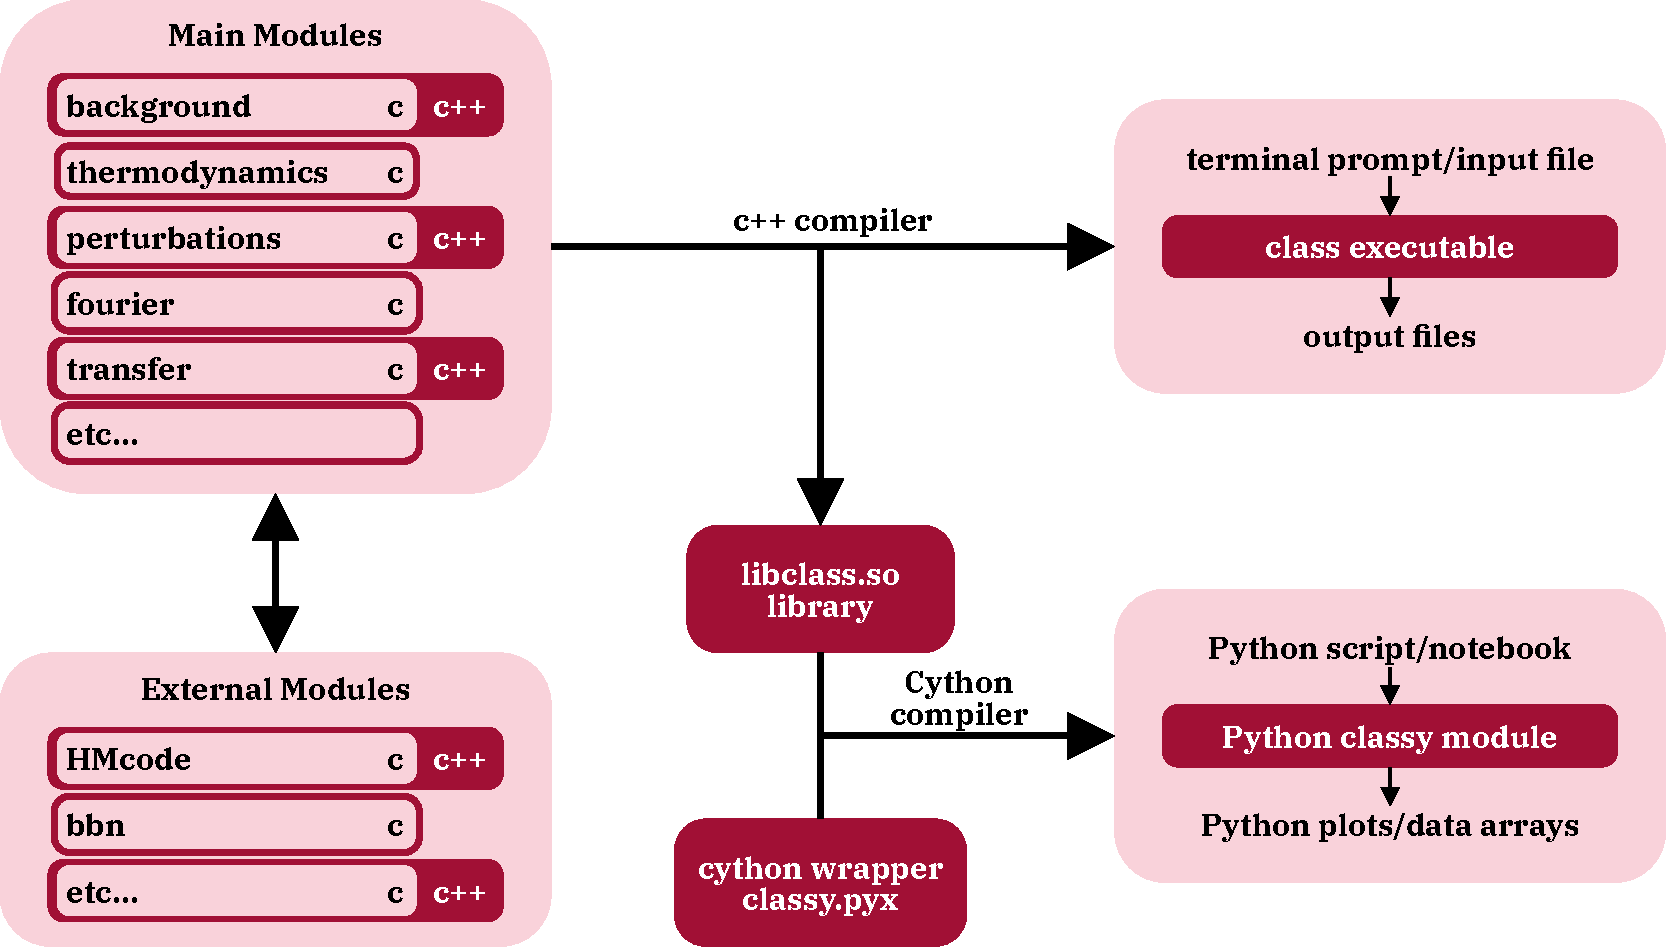
\includegraphics[width=\textwidth]{Figures/class_structure.pdf}

\end{frame}

\begin{frame}[fragile]
	\frametitle{\CLASS{} vs \classy{}}
	Let's clarify a bit of nomenclature!
	\begin{itemize}
		\item {\Red \CLASS{}} is the \texttt{C} code that does all the work of solving the EBS. It is used from the command line.
		\item {\Purple \classy{}} is the \texttt{Python} wrapper of {\Red \CLASS{}}, and internally uses it. It is used from a python interpreter.
	\end{itemize}
	The two share same input/output, except different naming and format
	(e.g. \mbox{\Red\texttt{.ini} file}  vs \texttt{\Purple python dictionary} as input)
\end{frame}

\begin{frame}[fragile]
\frametitle{Running \CLASS{} in terminal}

Run any input file with extension \cinline{*.ini}:
\hspace*{-2em}
\begin{itemize}
	\item Simple first-usage file \begin{class}
./class default.ini
	\end{class}
	\item Huge reference file containing all possible input parameters with comments
	\begin{class}
./class explanatory.ini
	\end{class}
	\item Slim file matching Planck 2018 "baseline model" bestfit \\ \begin{class}
./class base_2018_plikHM_TTTEEE_lowl_lowE_lensing.ini
	\end{class}
\end{itemize}
\pause
\begin{itemize}
	\item
	All input is presented in detail in \cinline{explanatory.ini} (apart from precision parameters)
	\item
	This is a \textit{reference} file; we advise you to not modify it: 
	\begin{itemize}
		\item {\scriptsize either start from a slim file (like {\tt default.ini}), }
		\item
		{\scriptsize or copy it and reduce it to a shorter and more friendly file, }
		\item {\scriptsize or write your own from scratch with only needed input lines.}
	\end{itemize}
\end{itemize}


\end{frame}



\begin{frame}[fragile]
	\frametitle{{\Red \CLASS{}} input parameters}
	The common 'language' for input is as follows
\begin{class}
parameter = value
\end{class}
with the python dictionary equivalent of
\begin{class}
{'parameter':'value'}
\end{class}
where value is passed as a {\Red \tt python string}.\\

\mbox{}\\

\pause
Special cases include
\begin{class}
option = yes/no
selection = a,b,c,d
\end{class}
and comments are
\begin{class}
parameter = value #comment behind parameter
#comment in its own line
\end{class}
\end{frame}




\begin{frame}[fragile]
	\frametitle{\CLASS{} vs \classy{}}
	\begin{center}
		Let's compare {\Red \CLASS{}} vs {\Purple \classy{}} for an execution:\\
		\mbox{}\\
		\begin{tabular}{c c}
			{\Red \CLASS{}} & {\Purple \classy{}} \\ \hline \rule{0pt}{3ex}
			{\Red \texttt{.ini} file} with & {\Purple \texttt{python dictionary}} with \\
			\texttt{parameter = value} & \texttt{'parameter':'value'} \rule[-1ex]{0pt}{0pt} \\ \hline 
			\multicolumn{2}{c}{Solving of equations in {\Red \CLASS{}}} \\ \hline \rule{0pt}{3ex}
			Output to {\Red files} & Output from {\Purple python functions} \\
			Options write files & Options enable functions \\
			& (otherwise error message) \\
			& \\ \hline \rule{0pt}{3ex}
			\cinline{./class myfile.ini}& \cinline{import classy}\\
			& \cinline{cosmo = classy.Class()} \\
			& \cinline{cosmo.set(mydictionary)} %\\
			% & \cinline{cosmo.compute()}
			
		\end{tabular}
	\end{center}
\end{frame}



\begin{frame}[fragile]
	\frametitle{Input parameters}
	If nothing given $\to$ {\Red Planck 2013 cosmology} with $\sum m_\nu = 0$\\ 
	\mbox{} \\
	Any parameter {\Red overwrites} the defaults (from {\Red \tt .ini file} or {\Purple \tt cosmo.set})\\
	\mbox{} \\
	Precision file {\Red \tt cl\_ref.pre} $\to$ close to `optimal' precision
\end{frame}



\begin{frame}[fragile]
	\frametitle{Input parameters}
	Most common/important parameters:
	\begin{itemize}
		\item \texttt{output = {\Red $\underbrace{\text{tCl}}_\text{Temperature $C_\ell^{TT}$}$, $\underbrace{\text{pCl}}_\text{Polarization $C_\ell^{TE/EE/BB}$}$, $\underbrace{\text{lCl}}_\text{Lensing $C_\ell^{\phi \phi}$}$}, {\Purple $\underbrace{\text{mPk}}_\text{Matter power $P(k,z)$}$, $\underbrace{\text{mTk}}_\text{Matter transfer $\delta_i(k,z)$}$, }
		$\underbrace{\text{vTk}}_\text{Velocity transfer $\theta_i(k,z)$}$,
		$\underbrace{\text{nCl}}_\text{Number count $C_\ell^{dd}$}$, 
		$\underbrace{\text{sCl}}_\text{Galaxy Lensing count $C_\ell^{ss}$}$ }
	\end{itemize}
\end{frame}

\begin{frame}[fragile]
	\frametitle{Input parameters}
	Most common/important parameters:
	\begin{itemize}
		\item \cinline{l_max_scalars = 2500}
		\item \cinline{P_k_max_1/Mpc = 1}
		\item \cinline{z_pk = 0, 1, 2}  for {\Red \tt class}
		\item \cinline{z_max_pk = 10}  for {\Purple \tt classy}
		\item \cinline{format = CAMB} for initial conditions
		\item \cinline{write_warnings = yes} for {\Red \tt class}
	\end{itemize}
\end{frame}


\begin{frame}[fragile]
	\frametitle{Input parameters}
	Most common/important parameters:
	\begin{itemize}
		\item \cinline{input_verbose = 1}
		\item \cinline{background_verbose = 2}
		\item \cinline{thermodynamics_verbose = 1}
		\item \cinline{perturbations_verbose = 1}
		\item \cinline{fourier_verbose = 1}
		\item \cinline{output_verbose = 1}
	\end{itemize}
	Verbosity parameters for {\Red \tt class}
\end{frame}


\begin{frame}[fragile]
	\frametitle{Input parameters}
	The $\Lambda$CDM parameters $\{H_0, A_s, n_s, \Omega_m, \Omega_b h^2, \tau_\mathrm{reio}\}$:
	\begin{itemize}
		\item Hubble constant\\
		\cinline{H_0=67}\\
		\cinline{h=0.67}\\
		\cinline{100*theta_s = 1.042}\pause
		\item Primordial amplitude\\
		\cinline{A_s=2.1e-9}\\
		\cinline{ln10^\{10\}A_s = 3.0} \qquad =$\ln(10^{10} A_s)$\\
		\cinline{ln_A_s_1e10 = 3.0} \\
		\cinline{sigma8 = 0.825} \qquad =$\int \frac{k^3 P(k,z=0)}{2\pi^2} T^2(k R_8) \mathrm{d} \ln k$\pause
		\item Primordial tilt\\
		\cinline{n_s=0.96}\pause
		\item Matter abundance\\
		\cinline{Omega_m=0.3}\\
		\cinline{omega_m=0.14} \qquad = $\Omega_m h^2$\\
		\cinline{Omega_cdm=0.25}\\
		\cinline{Omega_cdm=0.11} \qquad = $\Omega_\mathrm{cdm} h^2$\\
		\pause
		\item Baryon abundance\\
		\cinline{Omega_b=0.05}\\
		\cinline{omega_m=0.02233} \qquad = $\Omega_b h^2$\\
		\item Reionization time\\
		\cinline{z_reio=7.0} \\
		\cinline{tau_reio=0.05}\qquad  $\approx \int_0^{z_\mathrm{reio}} \sigma_T n_e \mathrm{d}\eta$\\
	\end{itemize}
\end{frame}


\begin{frame}[fragile]
	\frametitle{Input parameters}
	One-parameter extensions
	\begin{itemize}
		\item Curvature\\
		\cinline{Omega_k = 0}\\
		\item Dark radiation\\
		\cinline{N_ur = 3.044} $\equalhat N_\mathrm{eff}$\\
		\item CMB temperature\\
		\cinline{T_cmb = 2.7255}\\
		\item Lensing enhancement\\
		\cinline{A_L = 1}\\
		\item Primordial running\\
		\cinline{alpha_s = 0}\\
	\end{itemize}
\end{frame}

\begin{frame}[fragile]
	\frametitle{Input parameters}
	Dark Energy options
	\begin{itemize}
		\item Cosmological constant\\ \cinline{Omega_Lambda}
		\item Fluid \\ \cinline{Omega_fld}
		\item Scalar field \\ \cinline{Omega_scf}
	\end{itemize}
	\pause
	Universe is always filled (to be as curved as $\Omega_k$) by putting whatever dark energy is still available (If you want to fill with scalar field, you need \cinline{Omega_scf<0}).\\
	Using the Budget equation
	\begin{equation}
	\sum \Omega_i = 1+\Omega_k
	\end{equation}
	\pause
	\mbox{}\\
	Examples:\\
	% \hspace*{-8ex}
	\begin{tabular}{r c l}
		\cinline{Omega_m=0.3} &  $\Rightarrow$ & \cinline{Omega_Lambda -> 0.7} \\
		\cinline{Omega_fld=0.5,Omega_m=0.3} & $\Rightarrow$ & \cinline{Omega_Lambda -> 0.2} \\
		\cinline{Omega_Lambda=0,Omega_m=0.3} & $\Rightarrow$ & \cinline{Omega_fld -> 0.7} \\
		\makecell{\cinline{Omega_Lambda=0,Omega_fld=0,}\\ \cinline{Omega_scf=-1,Omega_m=0.3}} & $\Rightarrow$ &  \cinline{Omega_scf -> 0.7} \\
		\cinline{Omega_k=0.2,Omega_m=0.3} & $\Rightarrow$ & \cinline{Omega_Lambda -> 0.9}  \\
	\end{tabular}
\end{frame}

\begin{frame}[fragile]
	\frametitle{Input parameters}
	Neutrino mass
	\begin{itemize}
		\item \cinline{N_ncdm=1} (single massive neutrino)
		\item \cinline{m_ncdm=0.06} (in eV)
		\item \cinline{N_ur = 3.044 - 1.0132 N_ncdm = 2.0308} \\
		(each massive neutrino contributes 1.0132 to $N_\mathrm{eff}$ [QED corrections, could be optimized in future])\\
		or
		\item \cinline{Neff = 3.044} will automatically adjust \cinline{N_ur} to achieve the desired $N_\text{eff}$
	\end{itemize}
\end{frame}


\begin{frame}[fragile]
	\frametitle{Input parameters}
	Neutrino mass
	\begin{itemize}
		\item \cinline{N_ncdm=3} (three massive neutrinos)
		\item \cinline{m_ncdm=0,0.0495,0.0582} (inverted hierarchy)
		\item \cinline{N_ur = 3.044 - 1.0132 N_ncdm = 0.0044}\\
		or
		\item \cinline{Neff = 3.044} will automatically adjust \cinline{N_ur} to achieve the desired $N_\text{eff}$
	\end{itemize}
\end{frame}

\begin{frame}[fragile]
	\frametitle{Input parameters}
	Neutrino mass
	\begin{itemize}
		\item \cinline{N_ncdm=1} (one \textit{degenerate} massive neutrinos)
		\item \cinline{deg_ncdm=3} (triply degenerate)
		\item \cinline{m_ncdm=0.02} (total mass 0.06eV)
		\item \cinline{N_ur = 3.044 - 1.0132 N_ncdm * deg_ncdm = 0.0044} \\
		or
		\item \cinline{Neff = 3.044} will automatically adjust \cinline{N_ur} to achieve the desired $N_\text{eff}$
	\end{itemize}
\end{frame}

\begin{frame}[fragile]{Plotting}

\begin{columns}
	\column{0.9\textwidth}
	\begin{block}{You can get plots}
		\begin{enumerate}
			\item{Manually:} using the output files with e.g. {\tt gnuplot}, {\tt IDL}, {\tt python}, {\tt Mathematic}, {\tt GNU Octave}...
			\item{Automatically:} using {\tt \Red python} and script {\tt \Red CPU.py}, or {\tt MATLAB} and script {\tt plot\_CLASS\_output.m}
			\item{Interactively:} using \CLASS{} as a {\tt python} module, within a {\tt python} session or a {\tt \Red Jupyter Notebook}
		\end{enumerate}
	\end{block}
\end{columns}

\end{frame}


\begin{frame}[fragile]
	\frametitle{Running {\Red \CLASS{}} from Python}
	
	\begin{columns}
		\column{0.9\textwidth}
		\begin{block}{\CLASS{} as a {\tt Python} module}
			\begin{itemize}
				\item based on wrapper located in \cinline{python/classy.pyx} (developed initially by B.~Audren and extended by many others)
				\item the compilation produces a python module \cinline{classy.py} and installs it on your computer (can be called from anywhere)
				\item wrapper written in {\Red \tt Cython}, encapsulates most useful {\Red \CLASS{}} variables/functions, contains extra functions (e.g. MontePython-motivated)
				\item (project: get most of the wrapper generated automatically from C code at compilation - Coming soon!)
				\item goal: obtain, manipulate and plot the results directly within (i)python scripts or notebooks (recommended)
			\end{itemize}
		\end{block}
	\end{columns}
	
	% \begin{itemize}
	% 	\item we will now discuss several examples of scrips/notebooks which are available since \cinline{v2.7.0} in the folders \cinline{scripts/} and \cinline{notebooks/}
	% 	\item with \cinline{jupyter} installed, open the notebooks with e.g.
	% 	\begin{class}
	% 		jupyter notebook notebooks/warmup.ipnyb
	% 	\end{class}
	% 	\item if you can't make it with \cinline{jupyter}, you'll get the same results with
	% 	\begin{class}
	% 		python scripts/warmup.py
	% 	\end{class}
	% \end{itemize}
	
\end{frame}


% \begin{frame}[fragile]
% 	\frametitle{Existing {\tt \Red class} features}
% 	Let's say I want to run some cool model with {\Red \tt class} \pause
% 	\begin{center}
% 		\Large What's already in {\tt \Red class}?
% 	\end{center}
% \end{frame}

\begin{frame}[fragile]
 	\frametitle{Existing content already in \CLASS{}}
 	$\Lambda$CDM:
 	\begin{itemize}
 		\item {\Red Baryons} \texttt{Omega\_b}$=\Omega_b$ or \texttt{omega\_b}$=\Omega_b h^2$
 		\pause \item {\Red Cold Dark matter} \texttt{Omega\_cdm}$=\Omega_\mathrm{cdm}$ or \texttt{omega\_cdm}$=\Omega_\mathrm{cdm} h^2$ or \texttt{Omega\_m}$=\Omega_\mathrm{m}$ or \texttt{omega\_m}$=\Omega_\mathrm{m} h^2$
 		\pause \item {\Red Hubble} \texttt{H0}$=H_0$ or \texttt{h}$=h$ or \texttt{100*theta\_s}$=100\theta_s$
 		\pause \item {\Red Reionization} \texttt{z\_reio}$=z_\mathrm{reio}$ or \texttt{tau\_reio}$=\tau_\mathrm{reio}$
 		\pause \item {\Red Primordial Amplitude} \texttt{A\_s}$=A_s$ or \texttt{ln10\textasciicircum\_s}$=\ln(10^{10}A_s)$ or \texttt{sigma8}$=\sigma_8$
 		\pause \item {\Red Primordial tilt} \texttt{n\_s}$=n_s$
 	\end{itemize}
\end{frame}


\begin{frame}[fragile]
	\frametitle{Existing content already in \CLASS{}}
	Standard simple extensions:
	\begin{itemize}
		\pause \item {\Red Curvature} $\Omega_k$ (\texttt{Omega\_k})
		\pause \item {\Red Neutrinos} $m_\nu$ (\texttt{m\_ncdm}, \texttt{N\_ncdm}, {\color{purple} \texttt{N\_ur} adjustment} see \texttt{explanatory.ini})
		\pause \item {\Red Free-streaming dark radiation} $N_\mathrm{eff}$ (\texttt{N\_ur})
		\pause \item {\Red Helium abundance} $Y_p$ (\texttt{YHe})
		\pause \item {\Red Primordial running} $\alpha_s$ (\texttt{alpha\_s})
		\pause \item {\Red CPL Dark Energy} $w_0, w_a$ (\texttt{Omega\_fld}, \texttt{w0\_fld}, \texttt{wa\_fld}, {\color{purple} \texttt{Omega\_Lambda=0}?})
		\pause \item CMB temperature $T_\mathrm{cmb}$ 
	\end{itemize}
\end{frame}


\begin{frame}[fragile]
	\frametitle{Existing content already in \CLASS{}}
	Dark matter:
	\begin{itemize}
		\item Thermal Warm Dark Matter (\texttt{m\_ncdm}, \texttt{T\_ncdm}, \texttt{omega\_ncdm})
		\item Annihilating dark matter 
		\item Decaying dark matter (\texttt{Omega\_dcdmdr}, \texttt{Gamma\_dcdm})
		\item Non-trivial phase-space distribution (\texttt{ncdm} framework), neutrino flavor mixing, neutrino chemical potential
		\item Interacting with photons, baryons, neutrinos (\texttt{idm})
	\end{itemize}

	\pause
	Dark radiation:
	\begin{itemize}
		\item Fluid/Self-interacting (\texttt{idr})
		\item Viscous (\texttt{ceff2\_ur}, \texttt{cvis\_ur})
	\end{itemize}

	\pause
	Dark energy:
	\begin{itemize}
	\item CPL, EDE (\texttt{fld}) (this \texttt{EDE} is {\Red not} the usual EDE $\to$ \url{https://github.com/PoulinV/AxiCLASS} and \url{https://github.com/flo1984/TriggerCLASS} to be merged)
	\item Other fluid-like DE  (\texttt{fld})
	\item Quintessence/Scalar field   (\texttt{scf})
	\end{itemize}
\end{frame}


\begin{frame}[fragile]
	\frametitle{Existing content already in \CLASS{}}
	Thermal modeling
	\begin{itemize}
		\item Recfast recombination
		\item Hyrec-2recombination
		\item Tanh reionization
		\item Multi-tanh reionization
		\item Reionization from file
		\item Energy injection (PBH Evaporation,PBH Accretion,DM Decay,DM Annihilation)
		% \item Soon physical reionization model, 21cm
	\end{itemize}
	
	\pause
	Spectral distortions
	\begin{itemize}
		\item $y$ and $\mu$ distortions
		\item PCA of intermediate distortions
	\end{itemize}

\end{frame}



\begin{frame}[fragile]
	\frametitle{Existing content already in \CLASS{}}
	
	\pause
	Inflation/Primordial Powerspectrum
	\begin{itemize}
		\item Arbitrary potential $V(\phi)$
		\item Automatic finding of observable window
		\item Can impose inflation duration
		\item Tensor modes included automatically
		\item Read from file
	\end{itemize}

	\pause
	Initial conditions
	\begin{itemize}
		\item Isocurvature modes ($\nu$,$b$,$\mathrm{cdm}$)
		\item Synchronous/Newtonian gauges
	\end{itemize}

	\pause
	Nonlinear estimation/emulation
	\begin{itemize}
	\item Halofit
	\item HMcode 2016 and 2022
	\item Perturbation theory (very soon)
	\end{itemize}

	\pause
	Modified Gravity\\
	$\to$ {\Red HiCLASS} branch (Bellini, Sawicki, Zumalacarregui, \url{http://www.hiclass-code.net})
	
	\vspace*{0.5\baselineskip}
	\pause
	Extension to {\Red second-order perturbation theory}\\ SONG (Fidler, Pettinari, Tram, \url{https://github.com/coccoinomane/song})
\end{frame}

\begin{frame}[fragile]
	\frametitle{Fundamental layout of Einstein-Boltzmann solvers}
	\begin{tikzpicture}[
	start chain=going below,
	every join/.style={arrow,color=black},
	node distance=0.6cm
	]
	\node (bg) [process,on chain,join] {Homogeneous background\\
		$H(a),\rho_i(a),D(a),...$};
	\begin{scope}[start branch]
	\node (th) [process,on chain=going right,join] {Homogeneous thermodynamics\\
		$x_e(z),T_b(z),c_s(z),...$};
	\end{scope}
	\pause
	\draw[tuborg] let
	\p1=(th.north east), \p2=(th.south east) in
	($(\x1+0.5em,\y1)$) -- ($(\x2+0.5em,\y2)$) node[right,midway,xshift=2pt]  {Unify (?)};
	\pause
	\node (pt) [process,on chain,join] {Perturbations\\$\delta_i(k,\tau),\theta_i(k,\tau),...$};
	\begin{scope}[start branch]
	\node (pm) [process,on chain=going right,xshift=4.5em] {Initial condition\\ $P_\mathcal{R}(k)$};
	\end{scope}
	\draw[arrow,color=black] (pm) -- (pt) node[pos=0.4,cross=5pt,sloped] {};
	\draw[arrow,color=red] (pm) -- (pt) node[pos=0.48,sloped,label={[label distance=0.2em,color=red]270:Not required}] {};
	\pause
	\node (obs) [startstop,on chain,join] {Projection\\(LoS/fixed-time)};
	\node (sp) [process,on chain,join] {Correlation functions\\
		$P(k,z),C_\ell$};
	\draw[arrow,color=ForestGreen] (pm) |- (0pt,-70pt) -- (obs.north);
	\draw[arrow,color=black] (th.south) |- (60pt,-25pt)|- (pt.east);
	
	\pause \node [process, below=0mm of bg.north, anchor=north,fill=RWTHbordeaux,text=white] {Background module\\ \texttt{background.c}};
	\pause \node [process, below=0mm of th.north, anchor=north,fill=RWTHbordeaux,text=white] {Thermodynamics module\\ \texttt{thermodynamics.c}};
	\pause \node [process, below=0mm of pt.north, anchor=north,fill=RWTHbordeaux,text=white] {Perturbations module\\ \texttt{perturbations.c}};
	\pause \node [process, below=0mm of pm.north, anchor=north,fill=RWTHbordeaux,text=white] {Primordial module\\ \texttt{primordial.c}};
	\pause \node [startstop, below=0mm of obs.north, anchor=north,fill=RWTHbordeaux,text=white] {Transfer module\\ \texttt{transfer.c}};
	\pause \node [process, below=0mm of sp.north, anchor=north,fill=RWTHbordeaux,text=white] {Harmonic module \& Fourier module\\ \texttt{harmonic.c , fourier.c}};
	\pause \node [process, on chain, join,fill=RWTHbordeaux,text=white] {Lensing module \\ \texttt{lensing.c}};
	\pause \node [process, on chain=going right,fill=RWTHbordeaux,text=white] {Distortions module \\ \texttt{distortions.c}};
	\pause \node [process, on chain=going right,fill=RWTHbordeaux,text=white] {Input \& Output module \\ \texttt{input.c , output.c}};
	\onslide<1->
	\end{tikzpicture}
\end{frame}

% \begin{frame}
% 	\frametitle{Basic overview}
% 	\Large We now understand {\Red context \& usage} \\[0.5\baselineskip] $\to$ Let's give an {\Red overview} \\[2cm] (Full {\Purple theory \& coding} in cycle 2)
% \end{frame}


%\begin{frame}[fragile]
%\frametitle{Context}
%{\Red \CLASS{}} is the 5th public Einstein-Boltzmann solver covering all basic cosmology:
%\begin{enumerate}
%\item
%{\Red COSMICS} package in f77 (Bertschinger 1995)\\
%Basic equations, brute-force $C_l^{TT}$
%%\pause
%\item
%{\Red CMBFAST} in f77 (Seljak \& Zaldarriaga 1996)\\
%Line-of-sight, $C_l^{EE,TE, BB}$, open universe, CMB lensing
%%\pause
%\item
%{\Red CAMB} in f90/2000 (Lewis \& Challinor 1999)\\
%closed universe, better lensing, new algorithms, new approximations, new species, new observables...
%(\url{http://camb.info})
%%\pause
%\item
%{\Red CMBEASY} in C++ (Doran 2003)
%%\pause
%\item
%{\Red \CLASS{}} in C (Lesgourgues \& Tram 2011)\\
%simpler polarisation equations, new algorithms, new approximations, new species, new observables...
%(\url{http://class-code.net})
%\end{enumerate}
%... and there might still be 1 or 2 more!
%But only {\Red CAMB} and {\Red \CLASS{}} are currently developed and kept to high precision level.
%\end{frame}

%
%\begin{frame}[fragile]
%\frametitle{Module structure of {\Red \CLASS{}}}
%
%The \cinline{main(command-line-args)} function of CLASS located in \cinline{main/class.c} could only contain:
%\begin{class}
%int main(args) {
%  input_init(args,ppr,pba,pth,ppt,ptr,ppm,pha,pfo,ple,pop);
%  background_init(ppr,pba);
%  thermodynamics_init(ppr,pba,pth); 
%  perturbations_init(ppr,pba,pth,ppt);
%  primordial_init(ppr,ppt,ppm);
%  fourier_init(ppr,pba,pth,ppt,ppm,pfo);
%  transfer_init(ppr,pba,pth,ppt,pfo,ptr);
%  harmonic_init(ppr,pba,ppt,ppm,pfo,ptr,pha);
%  lensing_init(ppr,ppt,pha,pfo,ple);
%  distortions_init(ppr,pba,pth,ppt,pha,pfo,psd);
%  output_init(pba,pth,ppt,ppm,ptr,pha,pfo,ple,pop);
%  /* all calculations done, free the structures */
%  lensing_free(ple);
%  distortions_free(psd);
%  harmonic_free(pha);
%  transfer_free(ptr);
%  fourier_free(pfo);
%  primordial_free(ppm);
%  perturbations_free(ppt);
%  thermodynamics_free(pth);
%  background_free(pba);
%}
%\end{class}
%Of course we also need error management!
%\end{frame}







\end{document}
